\documentclass[11pt,a4paper,spanish]{book}
%\usepackage{estilo_unir}
\usepackage{biblatex}
% Imagenes
\usepackage{graphicx}
\graphicspath{ {./.images/} }
% Formato
\usepackage{float}
\usepackage{hyperref}
\usepackage[utf8]{inputenc}
\usepackage{comment}
\setcounter{secnumdepth}{3}

\addbibresource{./bibLib/referenceLib.bib}


\begin{document}
	%---------------------------
	%título del trabajo y autor
	%---------------------------
	\title{Reconocimiento y clasificación de emociones en la lengua no aprendidas}
	\author{Luisa Sánchez Avivar}
	%\date{d de mes de 2019}
	%\director{CiroRodríguez}
	%\nombreciudad{Lausanne}
	
	%---------------------------
	%marges
	%---------------------------
	%\usepackage[margin=1.9cm]{geometry}
	%---------------------------
	%---------------------------
	%---------------------------
	%---------------------------
	\chapter{Estado del Arte}
	\section{Contexto}
	El reconocimiento de emociones en el habla es una disciplina en inteligencia artificial que trata de reconocer y clasificar emociones a través de la señal de voz. Este campo de estudio se ha hecho cada vez más popular, pero su origen se remonta a 1996, desde que se presentara el primer trabajo defendible sobre el tema "Reconociendo emociones en el habla" de la mano de F.Daellert \cite{Dellaert1996}.
	Desde entonces, el reconocimiento de emociones a través de la voz ha sido motivo de interés para la investigación, sin embargo en su gran mayoría, se ha estudiado sobre un mismo lenguaje debatiendo la habilidad de reconocer y clasificar las emociones oralmente expresadas. 
	
	
	\subsection{Temas fonéticos}
	El objetivo del reconocimiento de emociones en el habla es reconocer el trasfondo emocional del mensaje a través de la voz. Esta manifestación sonora posee factores clave para la comunicación humana que ayudan en su interacción sin alterar el contexto del mensaje.\\
	
	La expresión de las emociones están íntimamente relacionadas con las propiedades fonéticas en el habla donde se observan señales y patrones para marcar contrastes lingüísticos en un idioma \cite{Pell2001} por lo tanto, los efectos del lenguaje en la comunicación emocional son evidentes al haber sido observadas y medidas, las variaciones en el rango tonal y la frecuencia para expresarlas, cambiando no sólo el tono si no también el patrón lingüístico asociado \cite{Davletcharova2015}.
	Por otro lado tanto la proporción de consonantes y vocales (que hacen variar la presión de aire que se necesita) como el ratio de sílabas por palabra en cada idioma, caracterizan la expresión oral de las emociones. Existen muchos factores relacionados con el lenguaje como la morfología o la duración del estímulo que podrían ser un impacto en la decodificación de los matices en la señal vocal, tal y como se explica en \cite{Chen2017}.
	Existe una clasificación dependiendo de la velocidad silábica en la expresión de dichos idiomas, sin embargo poco se conoce acerca de los efectos en las medidas respiratorias en el habla. Esta observación puede llevar a que se pregunte si en lenguajes tan dispares, las emociones expresadas mediante la voz puedan ser reconocidas desde el punto de vista del otro idioma.
	Normalmente estos estudios se llevan a cabo en un único lenguaje, lo que en el caso que nos acontece, se traduciría como el reconocimiento de emociones llevado a cabo en la lengua materna; Mientras este ejercicio puede llegar a ser intuitivo, distinguir las mismas emociones en la lengua extranjera supone un reto ya que implicaría importantes matices culturales. Por ejemplo, no sería lo mismo entender qué emociones intenta expresar un italo parlante desde el punto de vista de una persona que entiende el español (ambas lenguas latinas), que comprender las mismas emociones del discurso desde un germano hablante. Así bien, es importante definir qué idioma se está reconociendo y desde cuál, por lo que analizar las raíces lingüísticas y fonéticas de los idiomas a estudiar es esencial. \hfill \break
	
	\subsection{Reconocimiento del habla}
	De manera general y atendiendo a la manera de como modelar las emociones, la clasificación de emociones se ha tratado desde dos enfoques principales:
	\begin{itemize}
		\item Las emociones como categorías discretas
		\item Las emociones vistas a través de un modelo dimensional
	\end{itemize}

	En el primer punto, a todos los humanos se les atribuye un conjunto de emociones básicas que pueden ser reconocidas interculturalmente. El debate se centra en la definición de dichas emociones, y fue Paul Elkman y su equipo en 1992 \cite{Ekman1992} quien estableció que estas eran 6: enfado, asco, miedo , felicidad, tristeza y sorpresa.
	En el segundo punto, las emociones se definen respecto a una o más dimensiones, donde normalmente las dimensiones que se comprenden tienden a ser la afectividad, la excitación o la intensidad. Aquí la discusión se centra en encontrar el número de dimensiones que de lugar a un modelo coherente y pueda incluir las emociones conocidas. El modelo de Plutchik \cite{Plutchik2001} sea quizá el más conocido en este enfoque, y propone un modelo tridimensional que organiza las emociones en círculos concéntricos situando la más básicas en el centro. \hfill \break

	\subsubsection{Extracción de Características}
	La extracción de características es una de las secciones más importantes en el reconocimiento de emociones a través de la voz debido a la ambigüedad de las características y la variedad vocal. La extracción de características es el paso principal en el procesamiento del diálogo, y se lleva a cabo para centrarse en la información contenida en la señal y mejorar el grado de similitud y/o diferenciación entre las clases \cite{Hellbernd2016}. Hasta ahora, por lo general hay dos enfoques principales  con respecto al tipo de características usadas en el Reconocimiento de Emociones en el Discurso:\\
	Los rasgos prosódicos, los cuales extraen información de la prosodia, en concreto, tono, energía y duración, y por otro lado, las características del tracto vocal que normalmente indican la distribución de la energía en la frecuencia del rango vocal (conocidos como Coeficientes Cepstrales).
	La mayoría de los estudios centrados en este tema usan rasgos espectrales como la información extraída del tracto vocal, lo que supone obtener la información derivada del espectro de la señal de la voz y se usan para modelar los patrones de entonación y frecuencia del hablante \cite{Langari2020}.\\
	
	\begin{comment} 
		Buscar referencias para cada uno
		Añadir quiza STFT ?
		Hablar de la escala de Mel: http://practicalcryptography.com/miscellaneous/machine-learning/guide-mel-frequency-cepstral-coefficients-mfccs/
	\end{comment}
	
	En \cite{Rashid2018} se ofrece una breve explicación de cada una de las técnicas más comunes analizando sus puntos fuertes y débiles. Así pues, podemos encontrar la Transformada Wavelets Discreta (DWT) que a pesar de mejorar la información que se obtiene del diálogo en la correspondiente banda de frecuencia presenta variaciones indeseadas en los límites debido a que las señales de entrada son de una longitud finita. También podemos encontrar trabajos donde se usen Coeficientes de Predicción Lineal (LPC) los cuales hacen estimaciones bastante precisas al extraer las propiedades del tracto vocal, pero son altamente sensibles al ruido de cuantificación, por lo que demuestran no ser precisos cuando hay ruido de fondo. \\
	
	No obstante, a lo largo de los últimos años se ha popularizado el uso de otros métodos reportando mejores resultados, estos son:
	
	\paragraph{Coeficientes Cepstrales con Predicción Lineal (LPCC)}
	Calcula una envolvente a los Coeficientes de Predicción Lineal (LPC) y luego hace una conversión a coeficientes cepstrales; Tiene una baja vulnerabilidad al ruido de fondo y mejora el ratio de error en comparación a LPC, pero sigue teniendo una gran sensibilidad al ruido de cuantificación.\hfill \break
	
	\paragraph{Coeficientes Cepstrales en la escala de Mel (MFCC)}
	Se basa en la desintegración de la señal para tener como resultado un resumen de las características que la forman. La obtención de este conjunto de valores numéricos se basa por un lado, en el rango de frecuencias de Mel, el cual consiste en una adaptación de frecuencias de la señal a aquellas más fácilmente percibidas por el oído humano, y por lo otro lado, la separación de frecuencias mediante lo que llamamos cepstrales (\emph{Cepstrum}) que divide la señal en dos bandas de frecuencias: baja (correspondientes a los fonemas producidos por el tracto vocal) y alta (correspondientes a la excitación de las cuerdas vocales). \\
	Debido a esto, encapsula la mayor parte de energía proveniente del sonido que es generado por humanos, por lo que es frecuentemente usada y sugerida para identificar palabras monosilábicas en un discurso.\hfill \break
	
	Resumiéndolo, los objetivos clave, serían:
	\begin{itemize}
		\item Eliminar la excitación del tracto vocal.
		\item Independizar las características extraídas.
		\item Ajuste a como los humanos percibimos el ruido y la frecuencia del sonido.
		\item Capturar la dinámica fonética, que definirá el contexto.
	\end{itemize}
	
	MFCC constituye una perfecta representación para el sonido cuando la fuente es estable y consistente. 
	
	\begin{comment}
			Entre los más populares, (por ejemplo, \cite{Hajarolasvadi2019} y \cite{AbdulQayyum2019}) donde nos encontramos con los Coeficientes Cepstrales con Predicción Lineal (LPCC), que tras hacer una conversión a coeficientes cepstrales consiguen una baja vulnerabilidad al ruido de fondo en comparación con su predecesor LPC, y Coeficientes Cepstrales en la escala de Mel (MFCC), los cuales se basan en la desintegración de la señal para tener como resultado un resumen de las características que la forman. La obtención de este conjunto de valores numéricos se basa por un lado, en el rango de frecuencias de Mel, el cual consiste en una adaptación de frecuencias de la señal a aquellas más fácilmente percibidas por el oído humano, y por lo otro lado, la separación de frecuencias mediante \emph{Cepstrum} que divide la señal en dos bandas de frecuencias, baja (correspondientes a los fonemas producidos por el tracto vocal) y alta (correspondientes a la excitación de las cuerdas vocales). Debido a esto, encapsula la mayor parte de energía proveniente del sonido que es generado por humanos, por lo que es frecuentemente usada y sugerida para identificar palabras monosilábicas en un discurso\cite{Hajarolasvadi2019}.
		
	\end{comment}

	\subsubsection{Procesamiento de la señal como imagen}
	\begin{comment}
		TODO
		- En algunos trabajos hemos visto que blablabla y esto lleva a blablabla
		- En el auge de las redes convolucionales blablabla
		- Se debe referenciar
	\end{comment}
	
	No olvidemos que el tipo de dato con el que se trabajará principalmente serán señales, concretamente, de audio. En las señales de audio hay una cierta presión de aire que varía con respecto al tiempo, y al muestrearlas en un determinado rango de frecuencia, obtendríamos algo como lo siguiente:
	
	\begin{figure}[H]
		\centering
		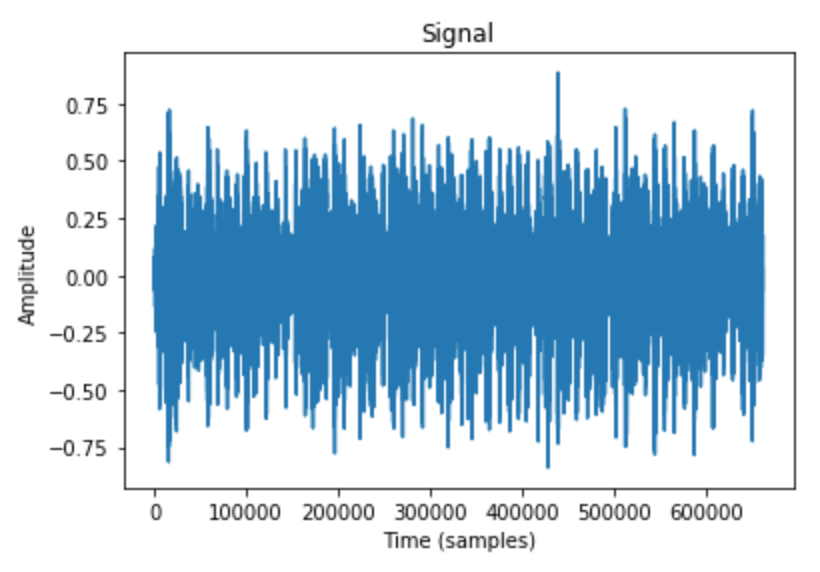
\includegraphics[scale=0.3]{waveform.png}
		\caption{Forma de onda de una señal de audio}
	\end{figure}
	
	Esto que vemos es una representación digital de la onda, de manera que ahora puede ser interpretada y analizada fácilmente.\hfill \break
	El siguiente punto que deberíamos atender, sería preguntarnos cómo extraer características relevantes de esta representación, y para ello encontramos la respuesta en la Transformada de Fourier (FFT \emph{Fast Fourier Transform}), la cual nos permite analizar la cantidad de frecuencia contenida en una señal. La Transformada de Fourier transforma la señal de un dominio de tiempo a un dominio de frencuencia, y el resultado de esta transformación se denomina espectro. \\
	Sin embargo el problema viene cuando en las señales de audio (que son el tipo de señales con las que queremos trabajar), la cantidad de frecuencia varía en el tiempo, por lo que FFT es insuficiente al no poder representar en el espectro resultante esta variación de la señal en el tiempo. La Transformada de Fourier en tiempo reducido, (\emph{short-time Fast Fourier Transform}) resuelve este problema calculando la FFT en segmentos (ventanas de tiempo) superpuestos de la señal. Lo que finalmente obtenemos se denomina \textbf{espectograma}.
	
	\begin{figure}[H]
		\centering
		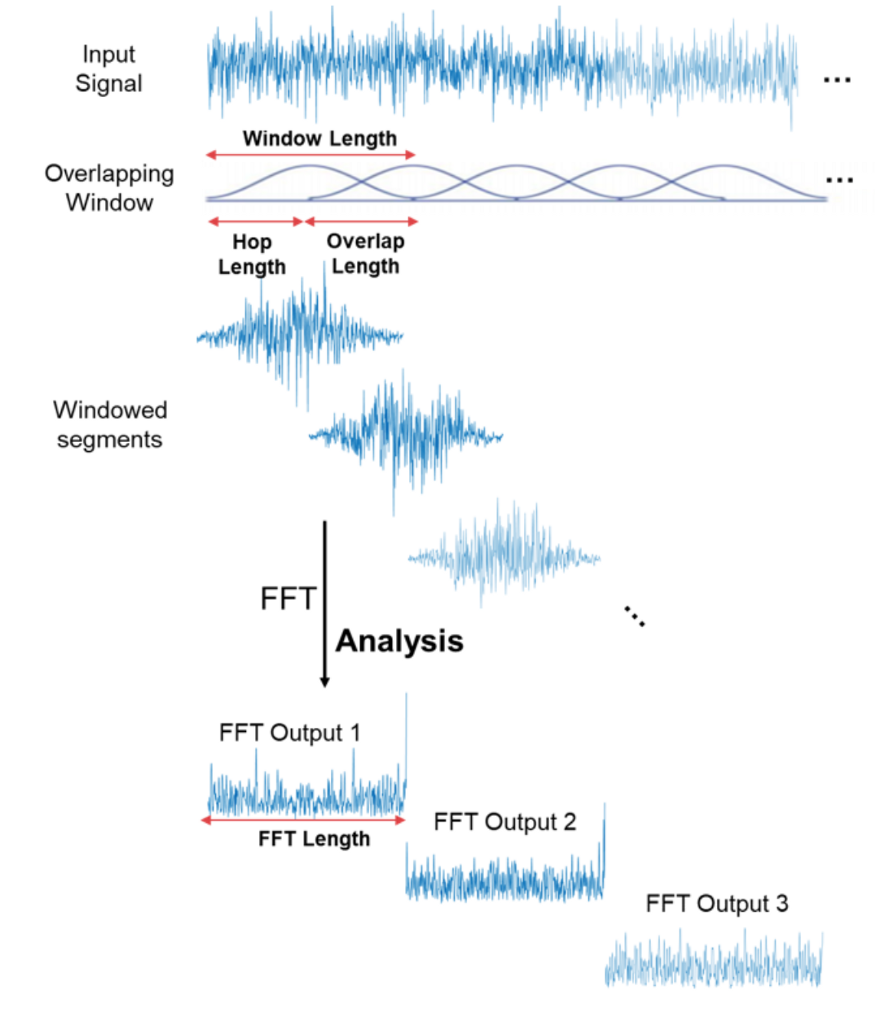
\includegraphics[scale=0.25]{processFFT.png} 
		\caption{Proceso del uso de FFT en una señal. Fuente: \href{https://www.mathworks.com/help/dsp/ref/dsp.stft.html}{Mathworks}}
	\end{figure} 
	
	
	Este espectograma puede ser entendido como una representación tridimensional de la señal donde sus características (tiempo, frecuencia y amplitud de la distribución de energía) pueden ser observadas de manera muy visual. Cuando este espectograma se computa, el eje X representa el tiempo, el eje Y representa la frecuencia, que es convertida a una escala logarítmica, y la gama de colores que se utiliza es para simbolizar la variación de energía expresada (medida decibelios), donde los tonos más oscuros indican unos valores de energía más altos, y viceversa.
	
	\begin{figure}[h]
		\centering
		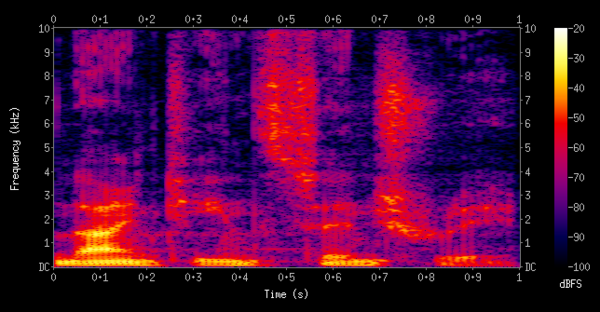
\includegraphics[scale=0.25]{spectogram.png} 
		\caption{Espectograma de una muestra aleatoria. Fuente: \href{https://es.other.wiki/wiki/Spectrogram}{Wiki}}
	\end{figure}
	
	La respuesta a por qué las frecuencias son convertidas a una escala logarítmica es sencillamente porque los humanos no percibimos las frecuencias en una escala lineal \cite{Varshney}, es decir, nuestra habilidad para distinguir entre frecuencias fluctúa a lo largo del rango en el que somos capaces de percibir\cite{StevensVolkmann}. Es por ello que el rango donde se mueve nuestro espectograma, se adapta a lo que se llama \textbf{escala de Mel}, en la cual los armónicos se observan equidistantes, reduciendo como resultado las variantes acústicas que no son significativas.\\
	
	Finalmente nos queda entender el concepto de \emph{Cepstrum} o coeficientes cepstrales, y para ello debemos entender como el sonido (respecto a la articulación de palabras) es producido. Técnicamente, esta producción del sonido en nuestra anatomía se definiría como la combinación de las vibraciones producidas por las cuerdas vocales con las vibraciones producidas por la resonancia del tracto vocal. Nuestras articulaciones controlan la forma del tracto vocal, por lo que la forma de onda (\emph{waveform}) de la voz será reprimida o amplificada a diferentes frecuencias por la forma de nuestro tracto vocal.\\
	El papel de Cepstrum es la separación de frecuencias en el algoritmo de MFCC, atendiendo a como los sonidos son producidos siguiendo un modelo anatómico, de manera que cuando es computado separa la señal de voz y la resonancia del tracto vocal. En \ref{fig:mfcc_process} observamos el paso IDFT, donde tras ajustar la señal a la escala de Mel, se calcula una variante de FFT (\emph{Inverse Discrete Fourier Transform}) y se obtienen los \textbf{coeficientes de MFCC}.
	
	\begin{figure}[h]
		\centering
		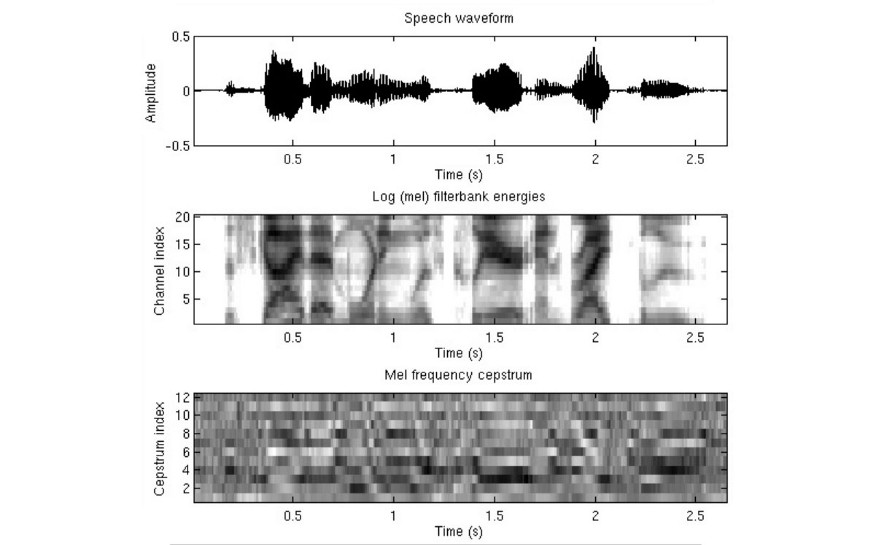
\includegraphics[scale=0.3]{waveform_process.jpeg} 
		\caption{Visualización de los coeficientes cepstrales de una muestra aleatoria. Aquí se puede observar el resultado de los pasos que hemos estado discutiendo hasta ahora. Fuente: \href{https://www.ee.columbia.edu/~stanchen/spring16/e6870/slides/lecture3.pdf}{Columbia University}}
	\end{figure}
	
	Dado que hemos convertido una señal de audio en una imagen, ahora se podrá proceder a usar un modelo basado en redes convolucionales, aprovechando sus ventajas en el campo donde mejor rendimiento reporta: el procesamiento de imágenes.
	
	
	\subsubsection{Algoritmos de Clasificación}
	
	\begin{comment} 
		Este parrafo debería ser referenciado
	\end{comment}
	Convencionalmente, el estudio del Reconocimiento de Emociones en el Habla incluye el uso de diferentes tipos de clasificadores para distinguir entre emociones: Suport Vector Machines (SVNs) los cuales se han usado extensamente
	para el reconocimiento de emociones y pueden llegar a presentar un buen rendimiento en comparación con otros clasificadores tradicionales, el algoritmo K-NN es de los enfoques más simples, Hidden Markov Model(HMM) es a menudo utilizado para lidiar con los cambios temporales en la señal y por último, Gaussian Mixture Model (GMM) el cual es útil para representar las unidades de sonido en características acústicas.%\cite{Farooq2020}.
	
	
	No obstante,en estudios más recientes, se han propuesto clasificadores basados en aprendizaje profundo y en redes neuronales densas (DNN) los cuales han superado a los enfoques tradicionales resultando ser más eficientes además de tener la capacidad de aprender las características emocionales en el reconocimiento de emociones a través del audio.
	
	\paragraph{Redes Neuronales Recurrentes}\hfill \break
	Las Redes Neuronales Recurrentes (RNN) son convenientes en tareas en las que los datos son procesados secuencialmente. Esto puede ser especialmente una ventaja ya que las distintas entradas de la señal no se tratan de manera independiente como se explica en \cite{Lim2017}. En \cite{Lee2015} se propone un sistema basado en RNN aprovechando esta particularidad donde cada nodo toma en cuenta la información recogida en los anteriores; Esto hace que cubra un espectro más amplio de información creando una especie de contexto.
	
	\begin{figure}[H]
		\centering
		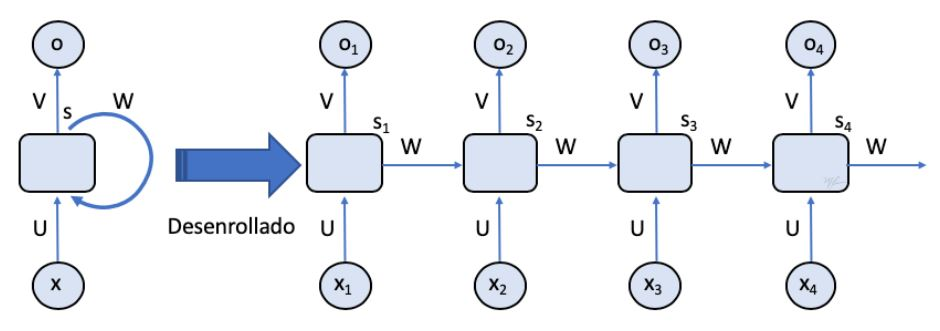
\includegraphics[scale=0.30]{rnn_structure.JPG} 
		\caption{Fuente:  \href{http://personal.cimat.mx:8181/~mrivera/cursos/aprendizaje_profundo/RNN_LTSM/introduccion_rnn.html}{Estructura de RNN}}
		\label{fig:rnn_structure}
	\end{figure}
	
	La figura \ref{fig:rnn_structure} muestra la estructura básica de una Red Neuronal Recurrente donde podemos observar como la red actualiza el peso de las entradas a través del algoritmo Descenso de Gradientes. En algunos casos, estos gradientes se irán haciendo más pequeños a medida que la red avanza, evitando así que los pesos cambien su valor y por lo tanto, la red siga aprendiendo. 
	
	\paragraph{Redes LSTM}\hfill \break
	Como podemos ver, los trabajos que implementan este tipo de arquitectura RNN son relativamente antiguos (2017, y 2015 respectivamente) y en trabajos más recientes , a destacar \cite{Wang2020} y \cite{Atmaja2019}, los retos que presenta la clasificación de emociones en el habla, son comúnmente abordados a través de una red de Memoria a Largo Corto-Plazo (LSTM) la cual es capaz de retener información de entradas anteriores en el tiempo y tener en cuenta dependencias temporales largas, ya que cada nodo es una célula de memoria. Esto a su vez, resuelve el problema de desvanecimiento de gradientes que presenta RNN.\\
	Las redes LSTM son un tipo de red recurrente que fueron diseñadas para resolver el problema de la dependencia a largo plazo del que sufre RNN. Como podemos ver en la figura \ref{fig:netLSTM}, estas presentan una estructura en cadena al igual que las redes recurrentes, pero el modulo de repetición en lugar de tener una única capa de red neuronal, tiene 4 que interactúan.
	\begin{figure}[H]
		\centering
		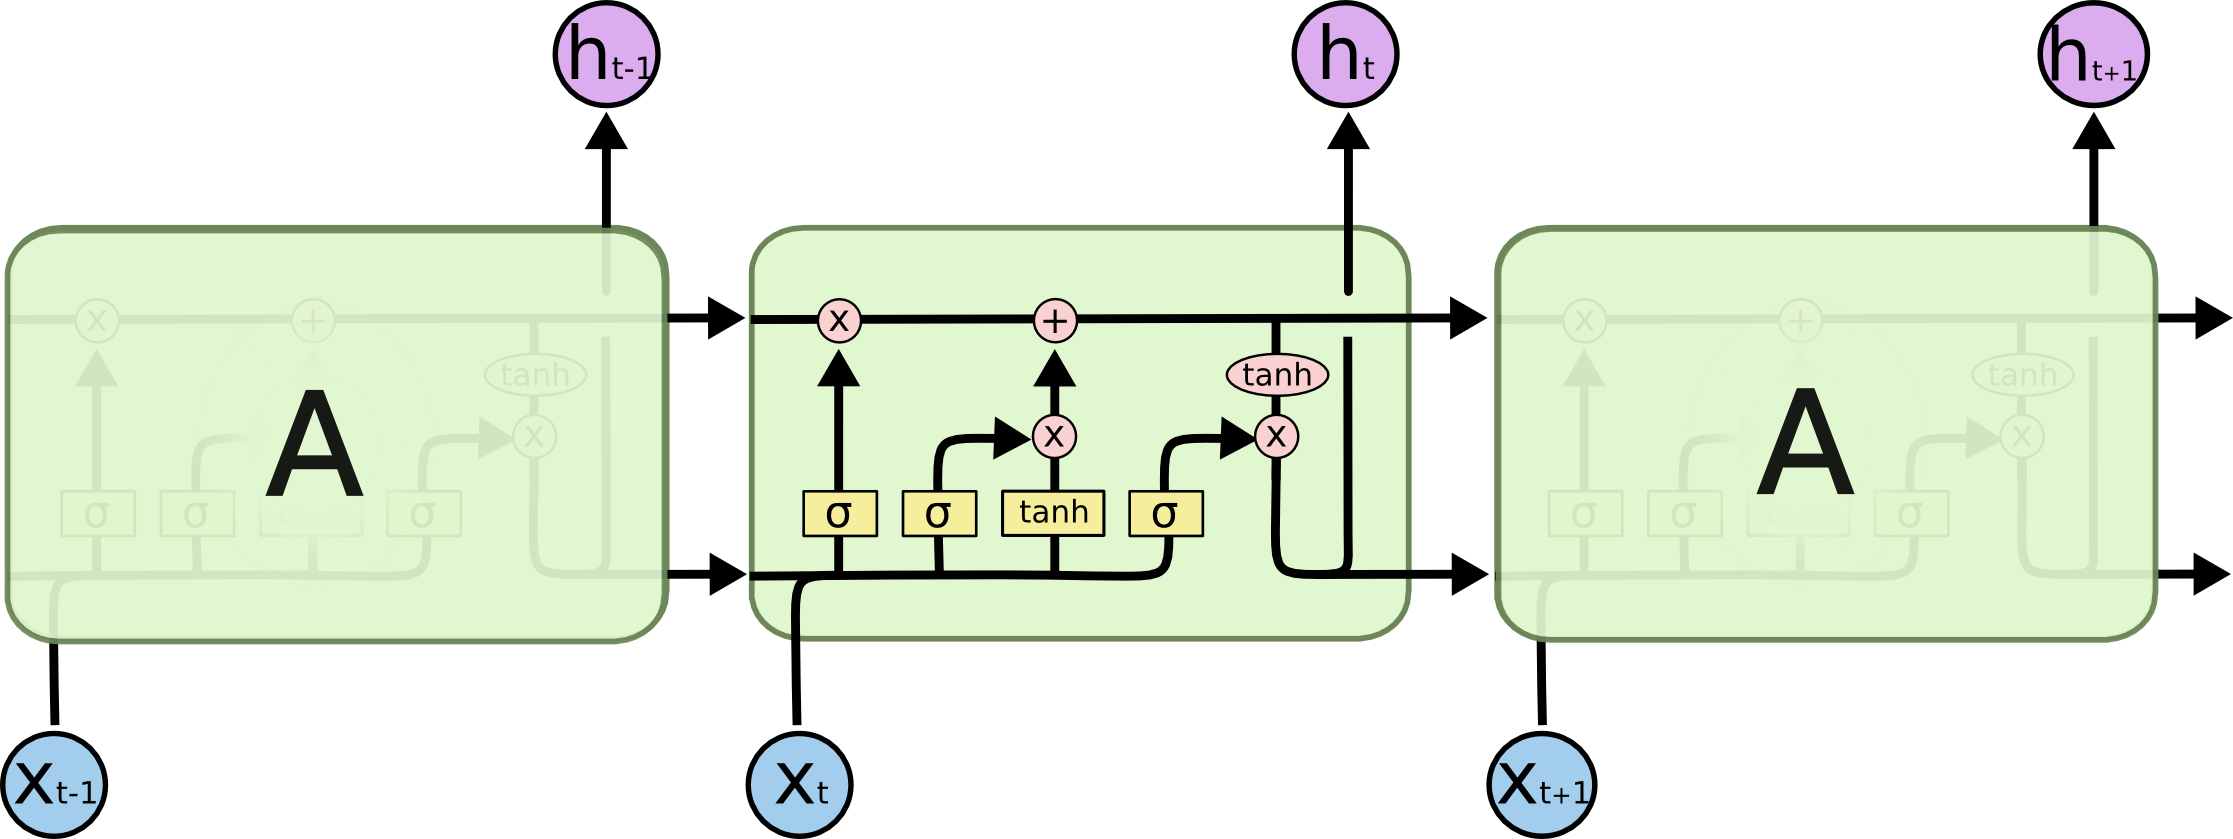
\includegraphics[scale=0.25]{LSTM3-chain.png}
		\caption{Estructura de una red LSTM. Fuente: \href{https://colah.github.io/posts/2015-08-Understanding-LSTMs/}{Colah}}
		\label{fig:netLSTM} 
	\end{figure}
	
	\paragraph{Redes Neuronales Convolucionales}\hfill \break
	Uno de los mayores avances de los últimos años en el campo de la inteligencia artificial son las redes convolucionales, debido a la alta precisión que proporcionan en el procesamiento de imágenes.
	
	La tendencia de los modelos basados en redes neuronales densas en este ámbito, es aprender características específicas desde varios métodos usados en el reconocimiento de emociones a través de la percepción acústica. En el uso de las Redes Neuronales Convolucionales (CNN) la idea principal es tomar ventaja de las propiedades de la señal, como la conectividad local, los pesos compartidos y el uso de varias capas  \cite{Lim2017}. Estas suponen una importante contribución en la Clasificación Emocional de la Voz debido al uso de características significativas, y su uso en recientes estudios se ha incrementado a lo largo de los años donde destacan los trabajos de \cite{AbdulQayyum2019} y \cite{Anvarjon2020}  %\cite{Farooq2020}.
	
	\subsubsection{Bases de datos}
	Aquí se recogen las bases de datos sobre el reconocimiento de emociones más usadas en los estudios comentados anteriormente.
	
	\begin{itemize}
		\item SAVEE (por sus siglas en inglés, \emph{ Surrey Audio-Visual Expressed Emotion}) es un conjunto de datos aplicado al reconocimiento de emociones que consiste en grabaciones de 480 frases en inglés británico ejecutadas por 4 actores profesionales masculinos modulando 7 emociones distintas (enfado, asco, tristeza, alegría, miedo, sorpresa y neutral). El estudio \cite{SAVEEdataset} explora y detalla esta base de datos que data del 2011, desgraciadamente su acceso está restringido.
		
		\item IEMOCAP (por sus siglas en ingles, \emph{Interactive Emotional Dyadic Motion Capture}) es una base de datos multimodal privada utilizada para el reconocimiento y análisis de emociones. Consiste en 12 horas de contenido audiovisual donde 10 actores (5 hombres y 5 mujeres) mantienen diálogos en ingles previamente transcritos en los que se interpretan 5 emociones distintas (enfado, tristeza, alegría, frustración y neutral).
		
		\item RAVDESS (por sus siglas en inglés, \emph{Ryerson Audio-Visual Database of Emotional Speech and Song}) es un popular conjunto dinámico multimodal (contiene varios formatos) donde 24 actores profesionales vocalizan frases en inglés norteamericano modulando 7 emociones (enfado, asco, tristeza, alegría, miedo, sorpresa y neutral). Tiene un total de 7356 grabaciones entre audio (hablado), audio(canciones) y vídeo. Es de acceso público.
		
		\item EMO-DB (por sus siglas en inglés \emph{Berlin Database of EMOtional speech}) es una base de datos alemana cuyos detalles se recogen en \cite{emodb2005}, data del 2005 y es de acceso público. La conforma una colección de 800 grabaciones interpretadas por 10 actores (5 hombres y 5 mujeres) matizando 7 emociones (enfado, asco, tristeza, alegría, miedo, sorpresa y neutral) y son llevadas a cabo en una cámara anecoica (capaz de absorber las ondas sonoras o electromagnéticas sin reflejarlas).
		
	\end{itemize}

	
	\begin{comment} 
	TODO
	Añadir más adelante las otras bases de datos
	\end{comment}
	
	\section{Estado del Arte}
	\label{lb_estado_arte}
	El reconocimiento de emociones en la voz es un área que ha sido estudiada a lo largo de los últimos años, sin embargo ese estudio se ha centrado en una sola lengua.
	No es despreciable el conocimiento que reportan [...]

	En \cite{Atmaja2019} proponen sistema basado en una arquitectura LSTM bidireccional (BLSTM) que aplican a un subconjunto de la base de datos IEMOCAP para distinguir entre cuatro emociones(enfado, excitación, tristeza y neutral). Discuten la incapacidad del un modelo BLSTM para detectar características relevantes, y palian el problema añadiendo un modelo de atención. Teniendo ese modelo como punto de partida (BLSTM + modelo de atención), experimentan escogiendo diferentes valores de duración del silencio para medir la eficacia que tendría el modelo si este se eliminara. Además utilizan un complejo sistema de extracción de características entre las que destacan MFCC. Los resultados muestran un máximo del 70.34\% de precisión en los datos sin necesidad de eliminar el silencio de la señal de audio.
	Un año después, J.Wang \cite{Wang2020} propone un modelo dual LSTM donde cada uterancia, se procesa con características MFCC y espectogramas de Mel simultáneamente. El modelo es entrenado y evaluado en el conjunto de datos IEMOCAP llegando a un 72.7\% de exactitud.
		
	Las redes LSTM cubren en mencionado antes, efecto de contexto, resolviendo el desvanecimiento de gradientes que podemos encontrar en las redes recurrentes, pero de manera aislada no son las que mejores resultados ofrecen y es por ello, que en otros trabajos se han combinado con CNN para aumentar su rendimiento. Por ejemplo en \cite{Lim2017} se lleva a cabo una comparación de tres  arquitecturas (CNN, LSTM y CNN distribuida en el tiempo) donde LSTM (utilizada de manera aislada) es la que puntúa más bajo. Al mismo tiempo, W.Lim y su equipo estudian el resultado de un sistema híbrido que usa una red convolucional distribuida en el tiempo (una combinación de CNN y LSTM) para clasificar emociones en una secuencia de audio, consiguiendo un 88.01\% de precisión. De nuevo, para aprovechar las ventajas que ofrecen las redes convolucionales, la señal es convertida a imagen (espectograma), que es entrenada y probada con el corpus EMO-DB (alemán) distinguiendo entre 7 emociones.
	
	Por otro lado, en \cite{Harar2017} describe un método que utiliza una arquitectura basada en Redes Convolucionales sin selección de características para distinguir únicamente entre tres emociones (enfado, neutral, y tristeza) a través de la voz. Su objetivo es predecir el estado emocional de una persona en una grabación corta de audio donde la mencionada arquitectura consiste en 6 capas convolucionales y 3 densas. Como conjunto de datos utilizan la Base de Datos de Berlín de Discurso Emocional (EMO-DB), un corpus alemán que contiene un total de 800 frases (10 frases distintas re-interpretadas en 7 emociones por 5 mujeres y 5 hombres), del cual extraen un subconjunto de 271 grabaciones etiquetadas. De las señales de audio con las que el sistema es alimentado, se han eliminado los segmentos de silencio después de ser estandarizadas consiguiendo una exactitud de 96.97\%.
	
	 Con el fin de eliminar el preprocesado de la señal, en \cite{AbdulQayyum2019}  presenta un modelo de redes convolucionales para una clasificación de emociones en el idioma inglés. Este utiliza la base de datos SAVEE, la cual contiene 480 muestras que distinguen entre 6 emociones, interpretadas por hombres y mujeres angloparlantes, donde obtiene finalmente un 81.63\% de precisión. Este trabajo llega a sus resultados mediante la comparación de 3 enfoques (MVR, SVN, y RNN) en el que a cada uno le aplican tres métodos de extracción de características distintos, con el sistema propuesto basado en CNN sin ningún procesado de la señal, siendo este último el que consigue una mejor capacidad de predicción.
	
	En estudios más recientes, \cite{Anvarjon2020} aborda el problema del Reconocimiento de Emociones en el Habla con una red CNN computacionalmente eficiente que es alimentada con los espectogramas de la señal; es decir, se consigue una representación en 2D de la señal de audio aprovechando mejor las ventajas de una red de este tipo. 
	\begin{figure}[H]
		\centering
		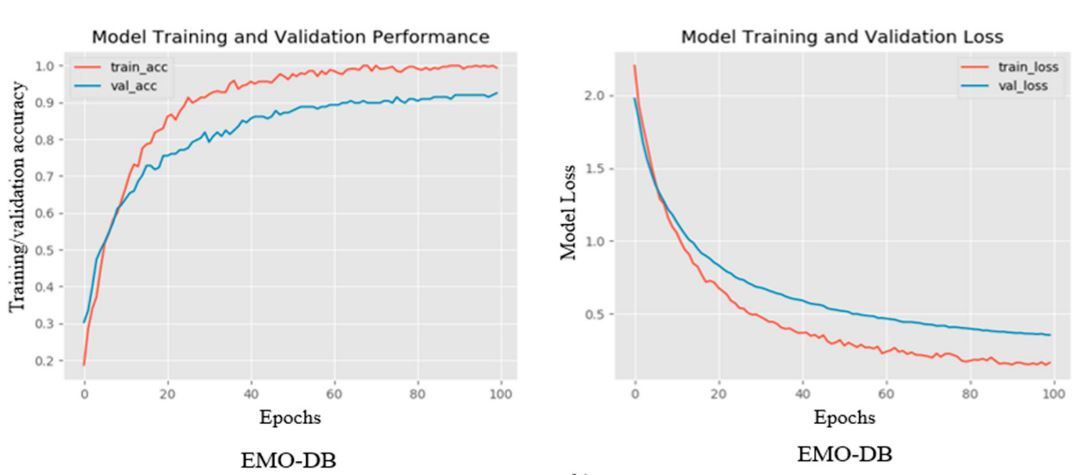
\includegraphics[scale=0.35]{anvarjon2020_emodb.JPG} 
		\caption{Resultados de T.Anvarjon sobre la base de datos EMO-DB}
		\label{fig:anvarjon_emo_plot}
	\end{figure}

	\begin{figure}[H]
		\centering
		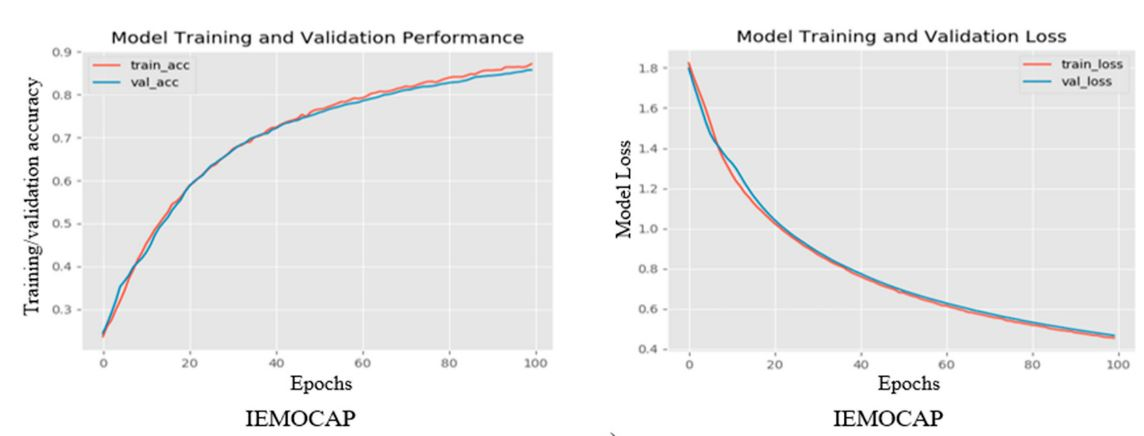
\includegraphics[scale=0.35]{anvarjon2020_imeocap.JPG} 
		\caption{Resultados de T.Anvarjon sobre la base de datos IEMOCAP}
		\label{fig:anvarjon_ime_plot}
	\end{figure}

	El sistema es probado en con dos datasets distintos independientemente, IEMOCAP (en inglés, y eliminando 'frustración') y EMO-DB (alemán) consiguiendo un 77.01\% y 92.02\%  de precisión respectivamente. En las figuras \ref{fig:anvarjon_emo_plot} y \ref{fig:anvarjon_ime_plot} vemos el rendimiento del modelo en los conjuntos de datos correspondientes comprobando el sólido resultado.
	
	
	\begin{comment}
		Finalmente, en \cite{Mustaqeem2021} exploran los efectos de la combinación de un mecanismo de atención junto a una red convolucional ligera. Al sistema se le pasa como entrada el espectograma de la señal y es probada en 3 datasets distintos: IEMOCAP (inglés),  RAVDESS (inglés), y EMO-B (alemán) consiguiendo un 78.01\%, 80.00\% y 93.00\% , para distinguir entre 4, 8 y 7 emociones respectivamente.
		
		
		Hablar del trabajo de https://arxiv.org/pdf/1912.10458.pdf
		
		Muy importante hablar de \cite{Tamulevicius2020}: En uno de los últimos estudios relacionados con este campo y que más que ver tienen con el tema que nos aborda, encontramos el trabajo de Tamulevicius donde lleva a cabo un estudio del reconocimiento emocional empleando el cruce de x lenguas blablabla
	\end{comment}
	
	 Siguiendo por el enfoque de CNN, en \cite{Mustaqeem2020} exploran una arquitectura basada en CNN compuesta por 7 capas bidimensionales. Paralelamente la red es alimentada con espectrogramas y características extraídas a través de MFCC, y lleva a cabo una clasificación de 5 emociones evaluando el resultado en RAVDESS donde consiguen un 81.0\% de precisión e IEMOCAP con un 84.00\%
	 
	 Finalmente, en una línea más cercana al objetivo de este proyecto es obligatorio hablar del trabajo de \cite{Tamulevicius2020} donde lleva a cabo un estudio del reconocimiento emocional empleando el cruce de 6 lenguas (lituano, inglés, serbio, español, alemán y polaco). La clasificación se lleva a cabo mediante el uso de una red neuronal convolucional bidimensional de 3 capas, e insisten en la importancia del uso de características en 2 dimensiones, ya que proveen información temporal además de las características acústicas de las emociones. En el estudio exploran varias de estas características, siendo el uso de cocleogramas las que consiguen una mayor exactitud.
	
	\section{Conclusiones parciales}
	En esta sección se valorarán las conclusiones que se extraigan del análisis previo sobre los distintas etapas correspondientes al desarrollo de un modelo para la clasificación de emociones en el habla. Vemos que los retos que plantea SER se han abordado anteriormente desde distintos enfoques, pero en su mayoría, desde el punto de vista de un único lenguaje. Las dificultades que presenta esta tarea en la lengua extranjera se deben principalmente a las posibles variaciones de aire para expresar la mismas emociones. Este mismo problema se plantea en una modalidad diferente pero bastante relacionada como es la transcripción de la voz a texto (ASR, Reconocimiento Automático del Discurso), sin embargo estos estudios requieren un estudio más en profundidad de la fonética propia de cada lenguaje.
	
	Los trabajos de Pell se han centrado durante años en el análisis de la prosodia a través de los idiomas. A pesar de su antigüedad y que no entra demasiado en detalles técnicos, merece la pena mencionar que en \cite{Pell2008} lleva a cabo un estudio comparativo entre la detección emocional de la prosodia en la lengua materna y la extranjera, concluyendo que el proceso para entender las emociones vocales en una lengua no aprendida, implica una mayor exposición a esta para familiarizarse con señales prosódicas correspondientes a significados subyacentes.\hfill \break
	
	Bajo estas líneas, podemos ver la tabla donde se resumen los estudios previamente comentados en la sección \ref{lb_estado_arte}.\\

	\begin{table}[H]
		\centering
		\begin{center}
			\begin{tabular}{| c | c | c | c| c | c|}
				\hline
					Trabajo & Año & Método &  Datos usados  & Acierto \\ 
				\hline
					Atmaja & 2019 &   BLSTM + Att  & IEMOCAP (4 emociones) & 73.34\% 	\\
					J.Wang & 2020 & LSTM dual + MFCC & IEMOCAP & 72.7\% \\
					W.Lim & 2017 &   LSTM + CNN & EMO-DB &  88.01\%		\\ 
					Harar & 2017 &  CNN & EMOD-DB (3 emociones) &  96.97\%			\\
					Abdul & 2019 & CNN & SAVEE & 81.63\%				\\
					Anvarjon & 2020 & CNN 2D + espectogramas Mel & IEMOCAP (4 emociones) & 77.01\%\\
					Anvarjon & 2020 & CNN 2D + espectogramas Mel & EMOD-DB & 92.02.01\%\\
					%Lim & 2017 & & & \\
					Mustaqeem & 2020 & CNN 2D + MFCC & RAVDESS (5 emociones) & 81.01\% \\
					Mustaqeem & 2020 & CNN 2D + MFCC & IEMOCAP (5 emociones) & 84.00\% \\  
					Tamulevicius & 2020 & CNN 2D + cocleogramas & Lithuanian & 97.00\% \\
					%& & & &
				\hline	
			\end{tabular}
		
			\caption{Tabla comparativa y resumida de los trabajos mencionados}
			\label{tab:metod_comp}
		\end{center}
	\end{table}

	En la tabla \ref{tab:metod_comp} se muestran un resumen de los estudios relacionados con este campo y sus correspondientes resultados, así como los métodos y datos que han usado para ello. La columna de Método, comprende la arquitectura completa, es decir, el sistema de clasificación usado y el método de extracción de características si lo hubiera. En la tercera columna se describen los datos usados (la base de datos) y el número de clases entre las que el sistema ha tenido que diferenciar.\\
	
	Cabe destacar que la combinación de métodos, veáse algoritmos de clasificación, filtros para preprocesar la señal, y métodos de extracción de características, así como distintos conjuntos de datos, es realmente diversa, por lo que visualizar una dirección clara para determinar qué línea es la mejor, se diluye. 
	
	No obstante hay observaciones, que pueden llevar a una conclusión general; Por ejemplo, y de manera intuitiva, cuanto mayor es el número de clases (emociones en nuestro caso), peor será la capacidad de clasificación de la red, y por eso en algunos trabajos se extrae un subconjunto reduciendo las opciones entre las que clasificar.  
	
	En la extracción de características el uso de MFCC ha sido amplia y tradicionalmente escogido al reportar resultados más elevados en comparación con otros métodos. En \cite{Langari2020} denota que los métodos de extracción de características son MFCC y LPCC porque las variaciones en la frecuencia del tono están significativamente relacionados con la expresión humana de emociones. Los parámetros que se computan en MFCC como el número de filtros o la escala de frecuencia, son a menudo escogidos de manera experimental y dependen en gran medida del conjunto de datos con el que se pruebe y el clasificador que implemente el sistema.
	
	Observamos también que CNN (con diferentes modificaciones dependiendo del estudio) es la opción más sólida entre los trabajos más recientes, debido principalmente a que reduce la señal de audio a sus características más relevantes, y la combinación de probabilidades resultantes identifica conjuntos de características que determinan una clasificación.
	
	\begin{comment} 
	Tal y como se muestra en el trabajo de J.Lee e I.Tashev \cite{Lee2015}, un sistema basado en una red neuronal densa puede no ser suficiente para cubrir el efecto contextual a largo plazo para interpretar las emociones en el diálogo (esto es, la necesidad de un contexto emocional previo en la prosodia para mejorar la clasificación en el tramo que se está actualmente analizando), por lo que este problema puede ser abordado desde una arquitectura RNN. Aún así
	
	 
	
	CNN es la opcion más sólida entre los trabajos más recientes
	
	Importante discusión sobre
	https://www.researchgate.net/post/Has-CNN-taken-over-RNN-in-Speech-Emotion-Recognition-If-yes-why
	
	Hablar del overfitting a pesar de una alta precisión
	\end{comment}
	
	\printbibliography
\end{document}